% main.tex -- CSMD-UTM article (design-oriented; no implementation or experiments)
% Compile: tectonic -X compile main.tex   (or: latexmk -xelatex main.tex)
\documentclass[12pt,a4paper]{article}
\usepackage[english]{babel}
\usepackage{csmd}          % unofficial reproduction of the CSMD-UTM Word template
\usepackage{amsmath}
\usepackage{tikz}
\usetikzlibrary{positioning,arrows.meta,fit,calc,backgrounds,shapes.misc}
\usepackage{pgfplots}
\pgfplotsset{compat=1.18}
\usepackage{algorithm}
\usepackage{algpseudocode}
\usepackage{xcolor}
\usepackage{enumitem}
\setlist{nosep,leftmargin=*}

\addbibresource{references.bib}

% ---- Edition-specific footer: fill in when the next CSMD edition is announced ----
\setcsmdfooter{Chisinau, [edition dates], Vol.~N}

% ---- Notation helpers ----
\newcommand{\Kr}{\mathcal{K}}
\newcommand{\Cset}{\mathcal{C}}
\newcommand{\Feas}{\mathcal{C}_{F}(w)}
\newcommand{\Vset}{\mathcal{V}}
\newcommand{\code}[1]{{\small\nolinkurl{#1}}}% breakable at / . _ ; write underscores unescaped

\begin{document}

\csmdtitle{Design of a Resource- and Network-Aware Cluster Selection Strategy for Karmada-Based Workload Placement}

% ---- Author block: verify name and replace placeholders before submission ----
\csmdauthors{Vasile CEBAN\textsuperscript{1*}}
\csmdaffiliation{\textsuperscript{1}[Department], group [GROUP], Faculty of Computers, Informatics and Microelectronics, Technical University of Moldova, Chisinau, Republic of Moldova}
\csmdcorresponding{*Corresponding author: Vasile Ceban, [EMAIL]}
\csmdtutor{Tutor/coordinator: [Given name FAMILY NAME], [scientific title], [affiliation]}

% Abstract: 150--200 words (template). Keywords: 4--6, alphabetical, lowercase, not repeating title terms.
\begin{csmdabstract}
Karmada places workloads on member Kubernetes clusters using cluster health, policy and capacity estimates, but it has no notion of the network latency between clients and clusters. This paper designs a cluster selection strategy that adds such latency to Karmada's existing scheduling process without replacing it. An analysis of the Karmada v1.19.1 source code shows four properties that constrain any extension: score plugins are summed without weights, scores influence selection only under a cluster spread constraint, capacity is estimated from requested rather than used resources, and placement is not revisited when cluster conditions change. Based on these properties, the design separates hard eligibility constraints, evaluated by a filter that reuses Karmada's replica estimators, from a soft score that combines post-placement resource headroom with normalised client-to-cluster round-trip time. Latency measurements are attached to cluster objects by an external probe and carry a validity rule: a cluster without a fresh measurement never benefits from the missing value, and the score falls back to resource-only ranking when no candidate has valid data. A worked example and an analysis of weight sensitivity illustrate the decisions of the design. A validation protocol for a future experimental study is proposed.
\end{csmdabstract}

\csmdkeywords{container orchestration, edge-cloud continuum, kubernetes federation, latency, scheduling plugin, telemetry staleness}


\section{Introduction}\label{sec:introduction}

Applications that serve users in several locations are increasingly deployed on more than one Kubernetes cluster. The clusters differ in capacity, in current load and in their network distance to the users. Orchestration across such clusters has been studied as part of the cloud-to-things continuum \cite{ullah2023orchestration}, and several systems coordinate independent clusters, among them the archived KubeFed project \cite{kubefed_repo}, Liqo \cite{iorio2023liquid} and Karmada \cite{karmada_repo,karmada_docs_architecture}. In Karmada, a central control plane receives a workload together with a propagation policy and decides on which member clusters the workload runs. This decision is made by the Karmada scheduler, which, unlike the Kubernetes scheduler, selects clusters rather than nodes.

The information used by this decision is limited. The Karmada scheduler evaluates API availability, cluster affinity, taints and an estimate of how many replicas each cluster can still accept. It does not use any measure of the network path between the clients of a workload and the candidate clusters. For latency-sensitive services, two clusters with equal free capacity can therefore receive the same preference although one of them is much farther from the clients. Tail latency matters in this setting, because response-time variability at the tail dominates the experience of interactive services at scale \cite{dean2013tail}.

Network-aware scheduling has been studied extensively at node level inside a single cluster \cite{santos2019networkaware,santos2023diktyo,wojciechowski2021netmarks,centofanti2023latency,ragavan2025nas}, and recent work has combined resource and latency information for selecting clusters \cite{tabatabaei2025cnf,bregar2026cosmospan,chiaro2024lais}. Combining the two kinds of information is therefore not new. What remains open, as discussed in \cref{sec:related}, is how such a combination fits into the mechanisms Karmada already provides. Existing proposals either delegate the decision to an external optimiser \cite{tabatabaei2025cnf} or replace Karmada's cluster scheduler with their own \cite{bregar2026cosmospan}. None of them specifies what happens when the network measurements are missing or out of date.

This paper addresses that question as a design study. It does not report an implementation or measurements; these are planned as a subsequent experimental study. The research questions are:
\begin{itemize}
  \item RQ1: How can resource and network information be incorporated into Karmada's cluster selection while keeping the existing scheduling behaviour as the foundation?
  \item RQ2: How should mandatory placement constraints be separated from optimisation objectives?
  \item RQ3: How can stale or unavailable network measurements be handled so that missing data is never treated as favourable?
  \item RQ4: Which trade-offs does the resulting design introduce?
\end{itemize}

The contributions of the paper are the following. First, it analyses the scheduling semantics of Karmada v1.19.1 at the level of the source code and identifies the properties that any custom cluster selection objective has to respect. Second, it proposes a design that keeps the hard eligibility conditions in Karmada's filter stage, reuses Karmada's own replica estimators for the capacity condition, and adds client-to-cluster round-trip time as a soft scoring signal with explicit validity and fallback rules. Third, it illustrates the decisions of the design analytically and proposes a protocol for validating it experimentally.

The paper is organised as follows. \Cref{sec:related} reviews related work. \Cref{sec:problem} formulates the problem. \Cref{sec:architecture} presents the architecture and \cref{sec:method} the cluster selection method. \Cref{sec:algorithm} describes the algorithm and its integration with Karmada. \Cref{sec:analysis} analyses the design, \cref{sec:validation} proposes the experimental validation, \cref{sec:limitations} states the limitations and \cref{sec:conclusions} concludes.

\section{Background and Related Work}\label{sec:related}

\subsection{Scheduling in Kubernetes and in multi-cluster systems}\label{sec:related-k8s}

Kubernetes inherited its scheduling model from cluster managers such as Borg, which places tasks on machines using admission control and resource packing \cite{verma2015borg}. The Kubernetes scheduler selects a node for each pod through a framework of plugins at defined extension points (filtering, scoring, reserving, binding and others), and the scores of the scoring plugins are combined using configurable weights \cite{k8s_scheduling_framework}. Surveys classify the large body of work that extends this scheduler by objective, workload type and environment \cite{carrion2022kubernetes,rejiba2022custom,senjab2023survey}. The most recent review covers 2023 to early 2026 and includes scheduling scopes from cloud to edge \cite{alhakimi2026enhancing}.

Placement across several independent clusters is a separate problem, because each cluster keeps its own control plane and its own node-level scheduler. KubeFed, the earlier federation project of the Kubernetes community, was archived in April 2023 \cite{kubefed_repo}. Liqo shares resources between clusters by representing a remote cluster as a virtual node of the local one \cite{iorio2023liquid}. Oakestra, an orchestrator for edge infrastructure that does not build on Kubernetes, uses a hierarchy in which a root component first selects a cluster and the selected cluster then places the task \cite{bartolomeo2023oakestra}. Karmada follows the same two-level decomposition while remaining Kubernetes-native: a central control plane selects member clusters, and the kube-scheduler of each member cluster selects nodes \cite{karmada_docs_architecture}.

\subsection{Karmada}\label{sec:related-karmada}

A workload submitted to Karmada is an ordinary Kubernetes resource template, for example a Deployment. A PropagationPolicy states the placement rules, such as cluster affinity, spread constraints and the replica scheduling type. The control plane combines template and policy into a ResourceBinding, the Karmada scheduler writes the selected clusters into that binding, and controllers then create the corresponding objects in the member clusters \cite{karmada_docs_architecture}. The scheduler can be extended with filter and score plugins compiled into a custom scheduler binary, and several scheduler instances can run side by side, each serving the workloads whose policy names it \cite{karmada_docs_custom_scheduler}. Rebalancing of workloads that are already placed is a separate, explicitly triggered mechanism \cite{karmada_docs_rebalancer}. An empirical study of Karmada has examined how applications are reconfigured after cluster failures or resource shortage \cite{patino2025reconfiguration}. The parts of the scheduler that matter for this paper are analysed in \cref{sec:karmada-analysis}.

\subsection{Network-aware scheduling within one cluster}\label{sec:related-node}

Santos et al.\ extended the Kubernetes scheduler to account for the round-trip time between nodes for fog applications \cite{santos2019networkaware}. Their later framework, Diktyo, places dependent microservices using an application dependency graph with latency and bandwidth requirements \cite{santos2023diktyo}; its plugins are distributed in the Kubernetes scheduler-plugins project \cite{schedulerplugins_networkaware}. NetMARKS scores nodes using metrics collected by the Istio service mesh \cite{wojciechowski2021netmarks}, and NAS uses latency and bandwidth observed through a Cilium eBPF service mesh \cite{ragavan2025nas}. Centofanti et al.\ argue for measuring latency at the application layer, as perceived by end users, instead of between cluster nodes \cite{centofanti2023latency}. Marchese and Tomarchio combine a network-aware scheduler plugin with a descheduler that moves pods when the network state or the traffic between microservices changes \cite{marchese2022ccgrid}, and they treat resource load in a separate strategy \cite{marchese2025loadaware}. Rossi et al.\ combine elasticity with network-aware placement for nodes that are geographically distributed but managed by one control plane \cite{rossi2020gekube}.

These works establish that network state is a useful scheduling signal, but they operate on nodes within one control plane. At cluster level the available resource information is aggregated over many nodes, it is refreshed periodically rather than observed per pod, and the relevant network path runs from clients to the entry point of a cluster rather than between nodes.

\subsection{Cluster selection with resource and network information}\label{sec:related-cluster}

Several works already combine resource and latency information when selecting clusters. Tabatabaei et al.\ build a service orchestration architecture on Karmada in which a filter plugin hands the candidate clusters to an external integer linear programming solver; the objective weighs peak CPU load against latency, and the authors state that the scoring mechanisms of Karmada are not yet included in their flow \cite{tabatabaei2025cnf}. Their simulation models latency with fixed round-trip values without running service traffic, and the authors name the focus on initial placement as a limitation. CosmoSpan selects a cluster and a node jointly through a multi-criteria scheduler that binds through the Karmada API, together with deschedulers that react to changes \cite{bregar2026cosmospan}. Its placement score covers CPU, memory, node uptime, bandwidth, latency and fault tolerance; it is evaluated mainly in simulation, and the Karmada scheduler is not part of the comparison because no simulation framework exists for it \cite{bregar2026cosmospan}. LAIS is a multi-cluster scheduler driven by end-to-end latency measurements that either meets a latency constraint or chooses the cluster with the lowest latency, and it is compared with the default Kubernetes scheduler \cite{chiaro2024lais}. Earlier, mck8s provided controllers on top of KubeFed that place, scale and burst applications across geo-distributed clusters and was evaluated on the Grid'5000 testbed \cite{tamiru2021mck8s}. The CODECO preprint ranks clusters using CPU, memory, bandwidth, latency and service class over Open Cluster Management \cite{sofia2026codeco}. Formal models for placement across federated domains also exist \cite{faticanti2023locality,khan2025latency}, as do learned policies based on deep reinforcement learning for multi-cluster scheduling \cite{huang2026kmps,jiang2025drkc}.

\Cref{tab:related} summarises how the closest works relate to the problem of this paper.

\begin{table}[t]
\caption{Cluster-level placement approaches that use resource and network information}\label{tab:related}
\centering\small\setstretch{1.0}
\begin{tabularx}{\textwidth}{@{}p{2.3cm}LLL@{}}
\toprule
\textbf{Work} & \textbf{Integration with orchestrator} & \textbf{Signals and decision} & \textbf{Missing-data handling, evaluation} \\
\midrule
Tabatabaei et al.\ \cite{tabatabaei2025cnf} & Karmada filter plugin calling an external ILP solver & Weighted peak CPU load and latency & Not specified; simulation with fixed RTT values, testbed deployment time \\
CosmoSpan \cite{bregar2026cosmospan} & Own scheduler; binds through the Karmada API & Multi-criteria score; latency as a filter & Not specified; KWOK simulation, multi-region overhead study \\
LAIS \cite{chiaro2024lais} & Multi-cluster scheduler with latency intents & End-to-end latency (hard or soft intent) & Not specified; comparison with the default Kubernetes scheduler \\
mck8s \cite{tamiru2021mck8s} & Controllers on KubeFed (archived) & Placement, scaling and bursting policies & Not specified; Grid'5000 testbed \\
CODECO \cite{sofia2026codeco} & Open Cluster Management & CPU, memory, bandwidth, latency, service class & Not specified; preprint without quantitative placement evaluation \\
This paper & Karmada filter and score plugins; default stages kept & Resource headroom and client-to-cluster RTT; capacity as a hard constraint & Explicit validity and fallback rules; design only, validation planned \\
\bottomrule
\end{tabularx}
\end{table}

Two observations follow from this comparison. First, none of the works defines how a decision is made when network measurements are missing or out of date, although measurements in a real system are periodic and can fail. Second, the works that build on Karmada either delegate the decision to an external solver or bypass the Karmada cluster scheduler, so the interaction of a resource- and network-aware objective with Karmada's own filtering, scoring and selection stages has not been described. This paper addresses both points at the design level. The empirical comparison against the default Karmada scheduler is left to the validation proposed in \cref{sec:validation}.

\section{Problem Formulation and Research Objectives}\label{sec:problem}

\subsection{Scheduling semantics of Karmada relevant to cluster selection}\label{sec:karmada-analysis}

The design is based on an analysis of the Karmada source code at release v1.19.1 (commit c64ba38) \cite{karmada_repo}. \Cref{tab:karmada} lists the properties that determine how a custom selection objective can be integrated. Each property is given with the source file in which it can be verified, so that the analysis can be repeated for later releases.

\begin{table}[t]
\caption{Properties of the Karmada v1.19.1 scheduler that constrain a custom cluster selection objective}\label{tab:karmada}
\centering\small\setstretch{1.0}
\begin{tabularx}{\textwidth}{@{}p{0.6cm}Lp{5.0cm}@{}}
\toprule
\textbf{ID} & \textbf{Property} & \textbf{Source file (under pkg/)} \\
\midrule
P1 & Extension points are Filter, Score and an optional NormalizeScore; no per-cycle state, reservation or extender interface exists. & \code{scheduler/framework/interface.go} \\
P2 & Plugins are compiled into the scheduler binary; the plugin factory receives no arguments. & \code{scheduler/framework/runtime/registry.go} \\
P3 & Scores of different plugins are summed without weights; a weight map exists but is never filled. & \code{scheduler/framework/runtime/framework.go} \\
P4 & An error returned by any plugin aborts the scheduling attempt. & \code{scheduler/framework/runtime/framework.go} \\
P5 & At initial placement both in-tree score plugins return 0. & \code{scheduler/framework/plugins/clusteraffinity/}, \code{.../clusterlocality/} \\
P6 & Without a spread constraint every feasible cluster is selected, independent of scores. & \code{scheduler/core/spreadconstraint/select_clusters.go} \\
P7 & Candidates are ordered by score, then by available replicas, then by name. & \code{scheduler/core/spreadconstraint/util.go}, \code{group_clusters.go} \\
P8 & If the top clusters lack capacity, the lowest-scored one is replaced by the remaining cluster with most available replicas, not by the next-best score. & \code{scheduler/core/spreadconstraint/select_clusters_by_cluster.go} \\
P9 & Available replicas are the minimum over the registered replica estimators; the estimator registry is exported. & \code{scheduler/core/util.go}, \code{estimator/client/interface.go} \\
P10 & Cluster resources are reported as Allocatable, Allocated and Allocating, all based on resource requests. & \code{controllers/status/cluster_status_controller.go} \\
P11 & Placement is not revisited when cluster status changes; only policy, replica or explicit triggers cause rescheduling. & \code{scheduler/scheduler.go}, \code{scheduler/event_handler.go} \\
\bottomrule
\end{tabularx}
\end{table}

Three consequences follow. Because of P3, weighting between resource and network criteria cannot be configured across separate plugins and has to be computed inside one plugin. Because of P6, scores only influence the outcome when the policy limits the number of selected clusters, for example to one. Because of P5 and P7, the default scheduler, for a new workload restricted to one cluster, selects the cluster with the largest estimated number of available replicas. The default behaviour is therefore already capacity-oriented, and it favours large clusters, since the criterion is an absolute replica count.

\subsection{Problem statement}\label{sec:problem-statement}

The paper considers the initial placement of a workload $w$ with $n_w$ replicas on exactly one member cluster. Single-cluster placement keeps all replicas, and therefore all communicating components of a single-tier service, in one cluster. Splitting a workload across clusters by score would require changes to Karmada's replica assignment rather than a plugin, and it is not considered here. The notation is summarised in \cref{tab:notation}.

\begin{table}[t]
\caption{Notation}\label{tab:notation}
\centering\small\setstretch{1.0}
\begin{tabularx}{\textwidth}{@{}p{3.1cm}Lp{3.2cm}@{}}
\toprule
\textbf{Symbol} & \textbf{Meaning} & \textbf{Unit / domain} \\
\midrule
$\Cset$, $\Feas$ & Member clusters; clusters eligible for $w$ & sets \\
$n_w$ & Number of replicas of $w$ & integer $\geq 1$ \\
$d_w^{k}$ & Request of one replica for resource $k \in \Kr = \{\mathrm{cpu}, \mathrm{mem}\}$ & millicores; bytes \\
$A_c^{k}$, $U_c^{k}$, $P_c^{k}$ & Allocatable, Allocated and Allocating amount of $k$ in cluster $c$ & as $d_w^{k}$ \\
$F_c^{k} = A_c^{k} - U_c^{k} - P_c^{k}$ & Free requestable amount of $k$ & as $d_w^{k}$ \\
$m_c(w)$ & Available replicas of $w$ in $c$ (minimum over estimators) & integer $\geq 0$ \\
$\ell_c$, $t_c$, $q_c$ & Client-to-cluster RTT (median), time of newest sample, number of samples & ms; s; integer \\
$\ell_{\mathrm{ref}}$ & RTT at which network suitability becomes zero & ms \\
$\tau$, $q_{\min}$ & Freshness horizon; minimum number of samples & s; integer \\
$\alpha$ & Weight of resource suitability ($1-\alpha$ for network suitability) & $[0,1]$ \\
$R_c(w)$, $N_c$, $S_c(w)$ & Resource suitability, network suitability, final score & $[0,1]$, $[0,1]$, $\{0,\dots,100\}$ \\
\bottomrule
\end{tabularx}
\end{table}

The selection problem is to choose
\begin{equation}\label{eq:selection}
c^{*}(w) = \arg\max_{c \in \Feas} S_c(w),
\end{equation}
where $\Feas$ contains only clusters that satisfy all mandatory conditions, and $S_c(w)$ expresses preferences among them. \Cref{eq:selection} thus separates the two kinds of criteria by construction: a cluster outside $\Feas$ cannot be selected whatever its score. Ties are resolved by the order of property P7.

\subsection{Research objectives and design requirements}\label{sec:requirements}

The research questions of \cref{sec:introduction} translate into the following design requirements.
\begin{itemize}
  \item D-R1 (integration): use only the documented extension mechanism (P1, P2) and keep the default Karmada stages unchanged, so that the extension can be disabled by selecting the default scheduler.
  \item D-R2 (separation): mandatory conditions are evaluated as filters and never traded against preferences; preferences are evaluated as scores.
  \item D-R3 (consistency): the capacity condition must agree with the capacity view used by Karmada's own selection stage, so that the replacement rule P8 does not override the ranking.
  \item D-R4 (safe telemetry): missing, malformed or stale network measurements must neither cause a scheduling error (P4) nor improve the score of a cluster.
  \item D-R5 (analysability): the score must be a closed-form function of observable inputs, so that decisions can be predicted and later tested.
\end{itemize}

\section{Proposed Architecture}\label{sec:architecture}

\Cref{fig:architecture} shows the proposed architecture. White components exist in Karmada and are used without modification. Shaded components are proposed in this paper. They are not implemented yet; the implementation is part of the planned experimental study.

\begin{figure}[t]
\centering
\IfFileExists{figures/architecture.png}%
  {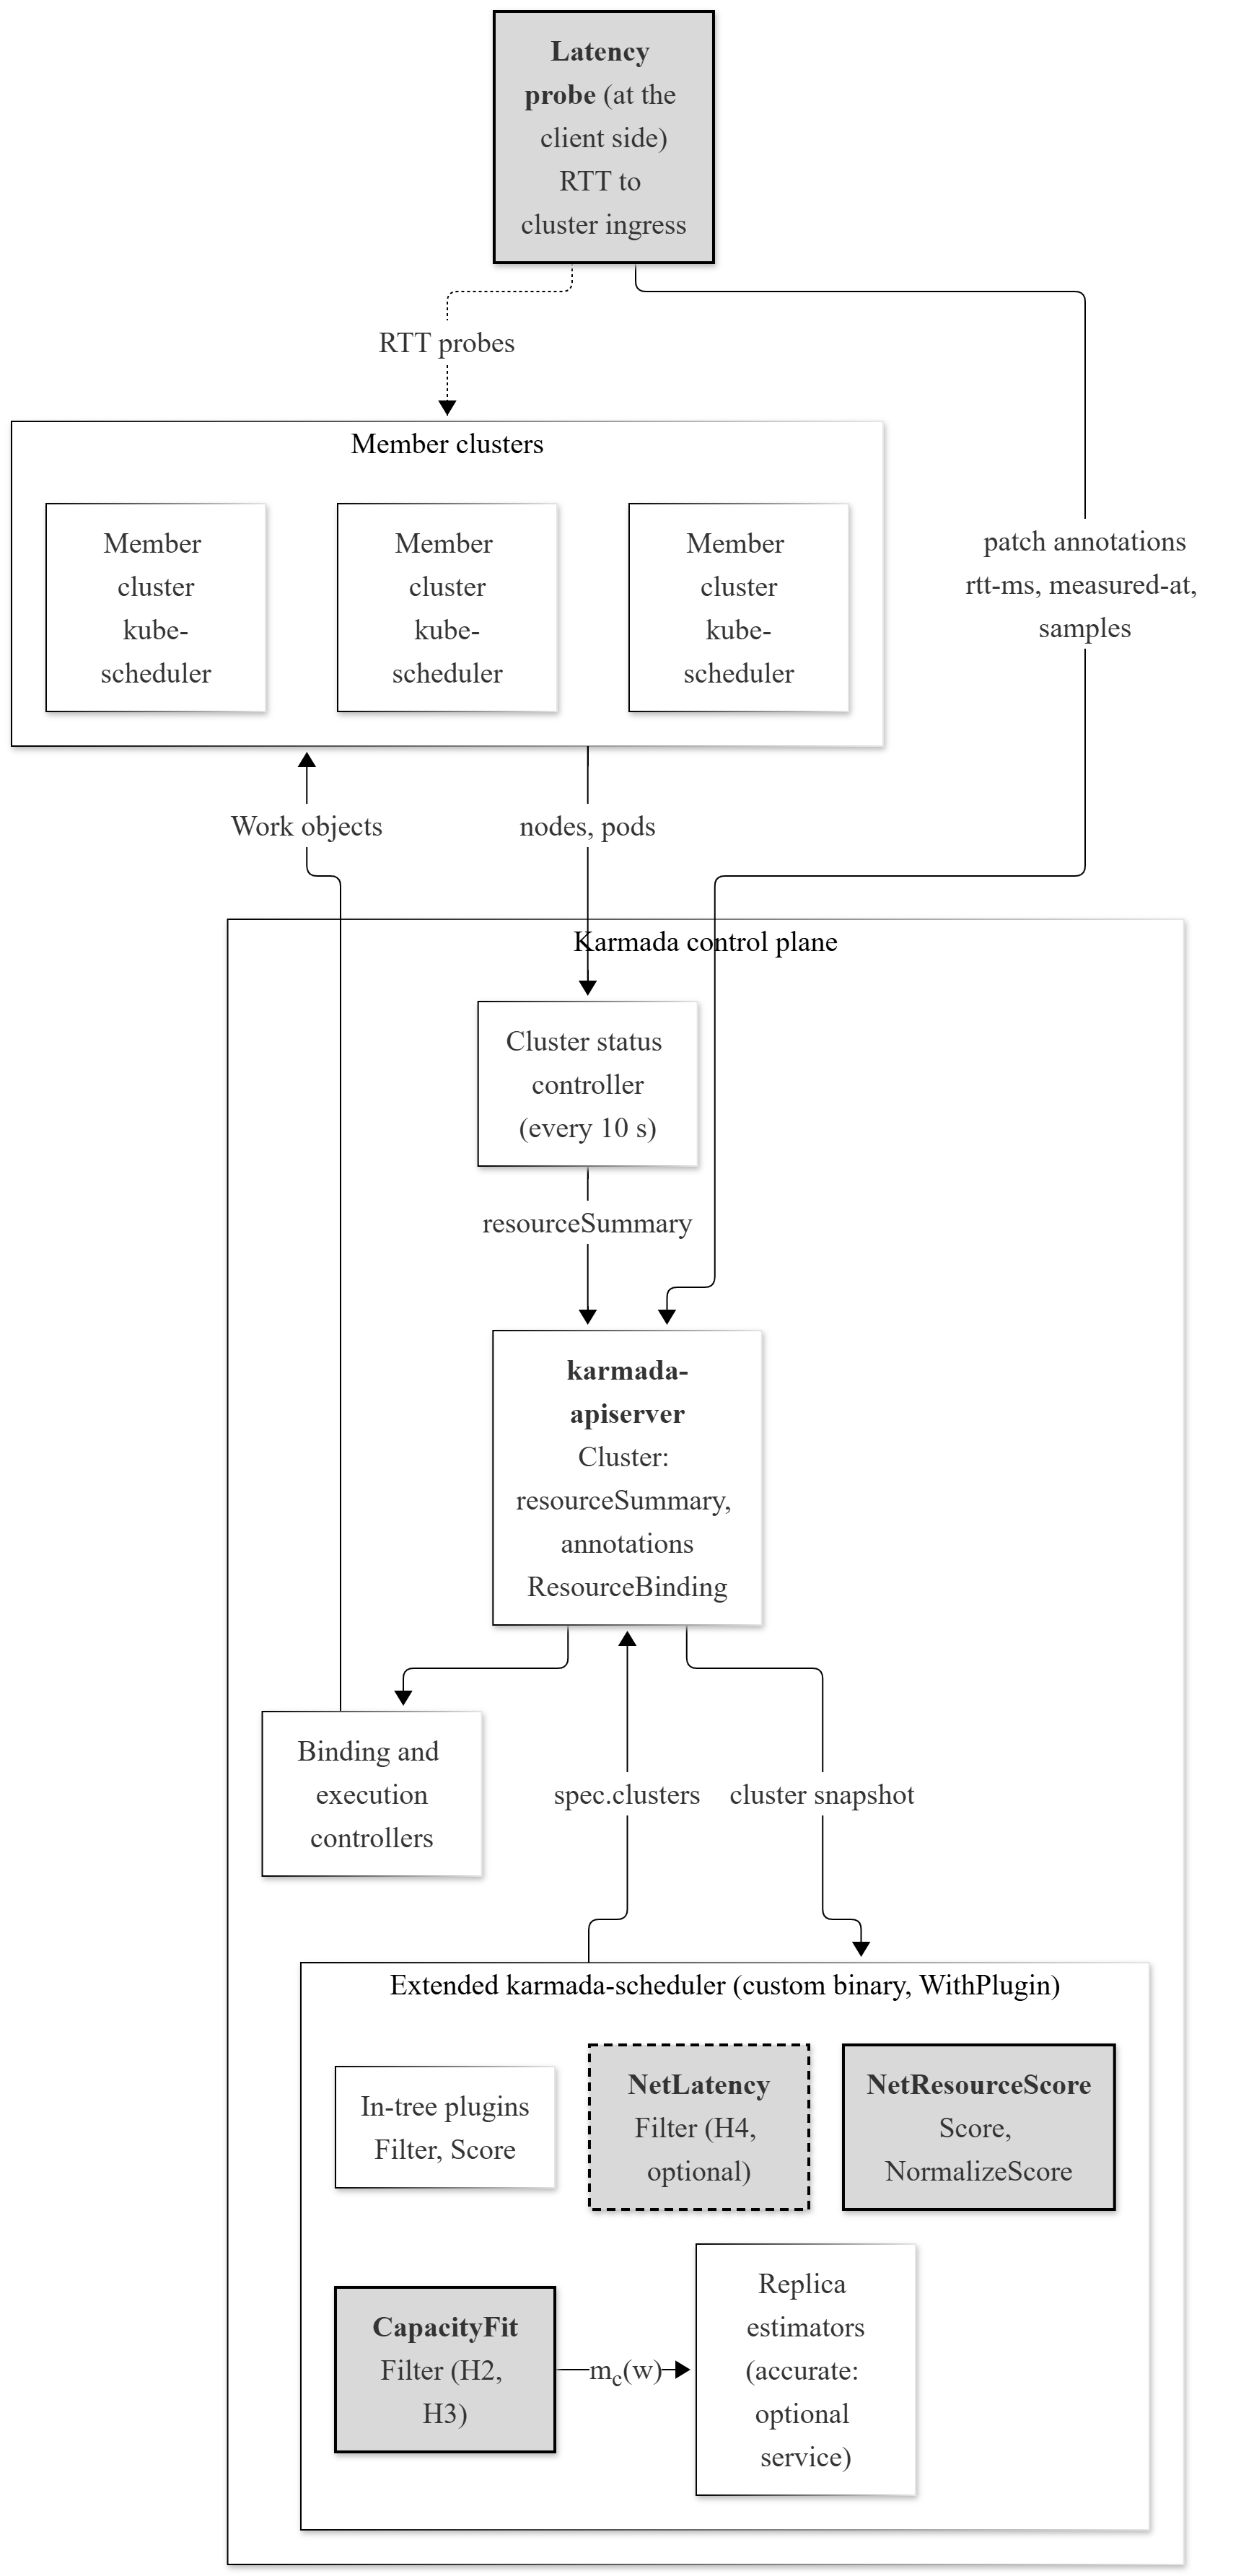
\includegraphics[width=\textwidth,height=0.7\textheight,keepaspectratio]{figures/architecture.png}}% exported from figures/mermaid/architecture.mmd
  {\resizebox{\textwidth}{!}{% Fig. 2 -- Proposed architecture. Shaded boxes = proposed components; white boxes = existing Karmada components.
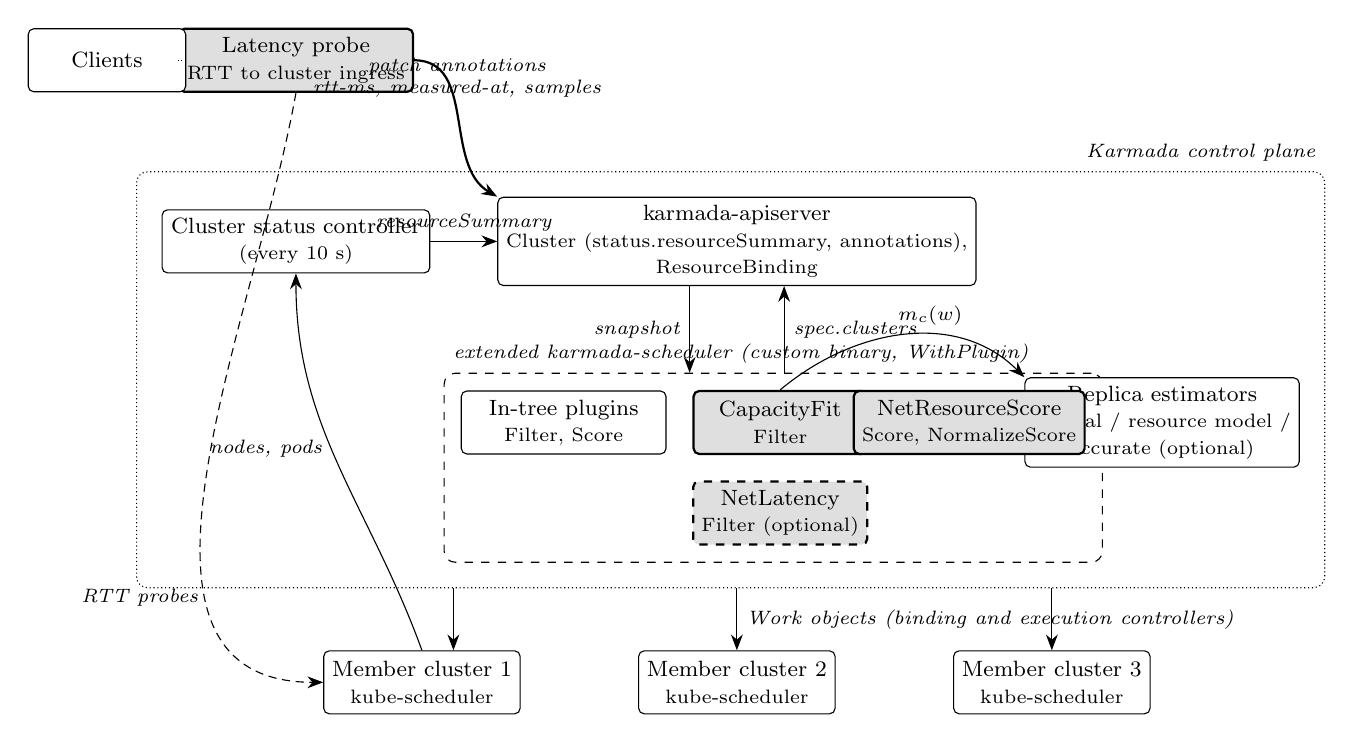
\begin{tikzpicture}[
  font=\footnotesize, >={Stealth[length=2mm]},
  box/.style={draw, rounded corners=2pt, align=center, minimum height=0.8cm, inner sep=3pt},
  prop/.style={box, fill=gray!25, thick},
  exist/.style={box, fill=white},
  grp/.style={draw, rounded corners=4pt, dashed, inner sep=6pt},
  lbl/.style={font=\scriptsize\itshape, align=center}
]
% ---------------- control plane ----------------
\node[exist, minimum width=4.6cm] (api) at (0,0) {karmada-apiserver\\ \scriptsize Cluster (status.resourceSummary, annotations),\\ \scriptsize ResourceBinding};
\node[exist, minimum width=3.4cm] (ctrl) at (-5.6,0) {Cluster status controller\\ \scriptsize (every 10 s)};
\node[exist, minimum width=3.0cm] (est) at (5.4,-2.3) {Replica estimators\\ \scriptsize general / resource model /\\ \scriptsize accurate (optional)};

% extended scheduler
\node[exist, minimum width=2.6cm] (intree) at (-2.2,-2.3) {In-tree plugins\\ \scriptsize Filter, Score};
\node[prop, minimum width=2.2cm] (cap) at (0.55,-2.3) {CapacityFit\\ \scriptsize Filter};
\node[prop, minimum width=2.4cm] (nrs) at (2.95,-2.3) {NetResourceScore\\ \scriptsize Score, NormalizeScore};
\node[prop, dashed, minimum width=2.2cm] (lat) at (0.55,-3.45) {NetLatency\\ \scriptsize Filter (optional)};
\begin{scope}[on background layer]
  \node[grp, fit=(intree)(cap)(nrs)(lat), label={[lbl, anchor=south west]north west:extended karmada-scheduler (custom binary, WithPlugin)}] (sched) {};
\end{scope}
\begin{scope}[on background layer]
  \node[grp, densely dotted, inner sep=9pt, fit=(api)(ctrl)(sched)(est), label={[lbl, anchor=south east]north east:Karmada control plane}] (cp) {};
\end{scope}

% ---------------- probe and clients ----------------
\node[prop, minimum width=2.6cm] (probe) at (-5.6,2.3) {Latency probe\\ \scriptsize RTT to cluster ingress};
\node[exist, minimum width=2.0cm] (clients) at (-8.0,2.3) {Clients};

% ---------------- member clusters ----------------
\node[exist, minimum width=2.4cm] (m1) at (-4.0,-5.6) {Member cluster 1\\ \scriptsize kube-scheduler};
\node[exist, minimum width=2.4cm] (m2) at (0.0,-5.6) {Member cluster 2\\ \scriptsize kube-scheduler};
\node[exist, minimum width=2.4cm] (m3) at (4.0,-5.6) {Member cluster 3\\ \scriptsize kube-scheduler};

% ---------------- data flows ----------------
\draw[->] (m1.north) to[out=110,in=-90] node[lbl, pos=0.55, left] {nodes, pods} (ctrl.south);
\draw[->] (ctrl.east) -- node[lbl, above] {resourceSummary} (api.west);
\draw[->, thick] (probe.east) to[out=0,in=150] node[lbl, above, pos=0.45] {patch annotations\\ rtt-ms, measured-at, samples} (api.north west);
\draw[->, densely dashed] (probe.south) to[out=-100,in=180] node[lbl, pos=0.7, left] {RTT probes} (m1.west);
\draw[-, densely dotted] (clients.east) -- (probe.west);
\draw[->] ([xshift=-6mm]api.south) -- node[lbl, left] {snapshot} ([xshift=-6mm]api.south |- sched.north);
\draw[<-] ([xshift=6mm]api.south) -- node[lbl, right] {spec.clusters} ([xshift=6mm]api.south |- sched.north);
\draw[->] (cap.north) to[out=40,in=135] node[lbl, above, pos=0.6] {$m_c(w)$} (est.north west);
\draw[->] (cp.south -| m2.north) -- node[lbl, right] {Work objects (binding and execution controllers)} (m2.north);
\draw[->] (cp.south -| m3.north) -- (m3.north);
\draw[->] ([xshift=4mm]cp.south -| m1.north) -- ([xshift=4mm]m1.north);
\end{tikzpicture}
}}% TikZ fallback
\caption{Proposed architecture; shaded boxes are proposed components, white boxes are existing Karmada components}\label{fig:architecture}
\end{figure}

\subsection{Components}\label{sec:arch-components}

The \emph{extended karmada-scheduler} is the standard Karmada scheduler built with three additional plugins through the documented out-of-tree registration (property P2) \cite{karmada_docs_custom_scheduler}. All in-tree plugins remain enabled. \emph{CapacityFit} is a filter that enforces the capacity condition by calling Karmada's replica estimators (P9). \emph{NetResourceScore} is a score plugin that combines resource headroom with network suitability; its normalisation step applies the validity rules for network measurements. \emph{NetLatency} is an optional filter for workloads that require a hard latency bound; it is disabled unless explicitly configured.

The \emph{latency probe} is an external controller placed close to the client population that a scheduler instance represents. It periodically measures the round-trip time to the service entry point of each member cluster, for example by timing a TCP connection set-up, and writes the result to annotations of the corresponding Cluster object in the Karmada control plane. The probe is not on the scheduling path: a failure of the probe changes only the validity of the stored measurements.

Monitoring systems such as Prometheus may observe the scheduler and the probe, but the decision does not query them. Querying an external service inside a score plugin would add network delay to every decision and could fail, and a failure aborts the scheduling attempt (P4).

\subsection{Telemetry contract}\label{sec:arch-telemetry}

The probe and the scheduler share the annotations listed in \cref{tab:telemetry}. Annotations are used instead of labels for a specific reason. A change of Cluster labels makes the scheduler re-enqueue the bindings whose cluster affinity can match the changed cluster, whereas a change of annotations triggers no re-enqueueing (P11). With measurements refreshed every few seconds, labels would cause continuous scheduling activity. The scheduler reads the current Cluster objects from its informer cache at the start of each decision, so annotations written by the probe are visible at the next decision without causing additional scheduling activity.

\begin{table}[t]
\caption{Cluster annotations written by the latency probe (prefix is a placeholder)}\label{tab:telemetry}
\centering\small\setstretch{1.0}
\begin{tabularx}{\textwidth}{@{}p{4.6cm}p{2.6cm}L@{}}
\toprule
\textbf{Annotation} & \textbf{Format} & \textbf{Meaning} \\
\midrule
\code{netaware.lab/rtt-ms} & decimal & $\ell_c$, median of the last $q_c$ samples, in ms \\
\code{netaware.lab/rtt-measured-at} & RFC 3339, UTC & $t_c$, time of the newest sample \\
\code{netaware.lab/rtt-samples} & integer & $q_c$, number of samples behind $\ell_c$ \\
\code{netaware.lab/rtt-vantage} & string & client population that the value represents \\
\bottomrule
\end{tabularx}
\end{table}

\subsection{Existing functionality and proposed extension}\label{sec:arch-existing}

\Cref{tab:existing} separates what Karmada provides from what the design adds. The extension does not modify Karmada's selection, replica assignment, propagation, rebalancing or failover mechanisms. A workload is handled by the extension only if its PropagationPolicy names the extended scheduler; all other workloads continue to use the default scheduler.

\begin{table}[t]
\caption{Existing Karmada functionality and proposed extensions}\label{tab:existing}
\centering\small\setstretch{1.0}
\begin{tabularx}{\textwidth}{@{}Lp{2.4cm}p{5.4cm}@{}}
\toprule
\textbf{Element} & \textbf{Existing} & \textbf{Role in the design} \\
\midrule
Filter/score framework, plugin registration, scheduler name & yes & used unchanged \\
Health taints and taint toleration filter & yes & mandatory condition H1 \\
Resource summary (Allocatable, Allocated, Allocating) & yes & input of resource suitability $R_c$ \\
Replica estimators & yes, in selection & also called before ranking (CapacityFit) \\
Spread constraint with \code{maxGroups}, tie-break order & yes & used unchanged \\
Client-to-cluster latency measurement & no & latency probe, annotations \\
Resource- and network-aware score with validity rules & no & NetResourceScore \\
Hard latency bound & no & NetLatency (optional) \\
Rebalancing, descheduling, failover & yes, separate & not modified \\
\bottomrule
\end{tabularx}
\end{table}

\section{Cluster Selection Methodology}\label{sec:method}

\subsection{Resource-capacity information available in Karmada}\label{sec:method-capacity}

Karmada's cluster status controller, or the Karmada agent for clusters in pull mode, lists the nodes and pods of each member cluster and writes three aggregate quantities to the Cluster object, by default every 10 s and only when they have changed \cite{karmada_repo}. \emph{Allocatable} $A_c^k$ is the sum of the allocatable amount of resource $k$ over all listed nodes, including nodes that are not ready or are cordoned. \emph{Allocated} $U_c^k$ is the sum of the resource requests of pods that are bound to a node and have not terminated, in all namespaces. \emph{Allocating} $P_c^k$ is the sum of the requests of pods that are not yet bound to a node. The request of a pod is the sum of its container requests, raised to the largest init-container request if that is higher, plus the pod overhead.

All three quantities describe requested, or reserved, resources. None of them reflects measured utilisation. This has three consequences for any decision based on them. Pods without requests contribute nothing, so a cluster loaded by such pods appears emptier than it is. Pending pods that will never fit still count in $P_c^k$, which is conservative. Nodes that cannot accept pods still count in $A_c^k$, which is optimistic. The design uses this information anyway, because it is the same request-based view that Kubernetes uses to admit pods to nodes, it is already present in the scheduler's cache, and it does not depend on an external monitoring system.

Aggregate quantities do not show fragmentation. A pod must fit on a single node, so a free amount $F_c^k \geq d_w^k$ does not guarantee that one replica fits. Karmada's replica estimators handle this to different degrees. The general estimator divides the free aggregate amount by the per-replica request when no resource models are available. When resource models are enabled, which is the default, each node is assigned to a grade according to its free resources and represented by the lower bound of that grade, which is conservative. With the default grade boundaries, a node with less than one free CPU or less than 4 GiB of free memory falls into the lowest grade, whose lower bound is zero, and contributes no capacity. Clusters built from small nodes are therefore underestimated unless finer resource models are configured. An optional accurate estimator simulates node-level placement inside each member cluster through a remote call. Disabling the controller option \code{enable-cluster-resource-modeling} is not a way to switch the models off: it stops the collection of the whole resource summary, after which the estimate becomes zero. The models are controlled by a separate feature gate.

\subsection{Mandatory eligibility constraints}\label{sec:method-hard}

A cluster belongs to the eligible set $\Feas$ only if all of the following conditions hold. They are evaluated in the filter stage, before any score is computed.
\begin{itemize}
  \item H1 (existing): the cluster serves the API of the workload, matches the cluster affinity of the policy, and has no taint that the workload does not tolerate. Unhealthy clusters receive \code{not-ready} or \code{unreachable} taints automatically, so health is covered by this condition.
  \item H2 (capacity): the whole workload fits,
  \begin{equation}\label{eq:capacity}
    m_c(w) = \min_{e \in E} \widehat{m}_{c}^{e}(w) \geq n_w,
  \end{equation}
  where $E$ is the set of replica estimators registered in the scheduler and $\widehat{m}_{c}^{e}(w)$ is the estimate of estimator $e$.
  \item H3 (data presence): the resource summary of the cluster exists. Otherwise $m_c(w) = 0$ and H2 fails.
  \item H4 (optional latency bound): if a hard bound $\ell_{\max}$ is configured, the measurement of $c$ must be valid in the sense of \cref{sec:method-validity} and $\ell_c \leq \ell_{\max}$.
\end{itemize}

The condition in \cref{eq:capacity} uses the same estimators that Karmada's selection stage uses, as required by D-R3. Without H2 in the filter stage, a top-scored cluster that lacks capacity would be replaced by the cluster with most available replicas (P8), which discards the ranking. With H2, the clusters that reach the scoring stage are those that the selection stage would also accept. Fragmentation is handled to the extent provided by the configured estimator; the plugin does not re-implement node-level fitting.

H4 is evaluated fail-closed: a cluster without a valid measurement is not eligible. A hard bound is a guarantee, and a guarantee cannot be checked without data. H4 is therefore kept out of the default configuration, in which latency is only a preference.

\subsection{Resource suitability}\label{sec:method-resource}

Resource suitability is the fraction of the bottleneck resource that remains free after the workload is placed:
\begin{equation}\label{eq:resource}
  R_c(w) = \operatorname{clip}\!\left( \min_{k \in \Kr} \frac{F_c^{k} - n_w\, d_w^{k}}{A_c^{k}},\ 0,\ 1 \right).
\end{equation}
The minimum follows the resource that limits the cluster, so a cluster with free CPU but little free memory does not obtain a high value. Normalising by $A_c^k$ makes the value independent of cluster size. This is the intended difference from the default tie-break (P7), which prefers the cluster with the largest absolute number of available replicas and therefore tends towards large clusters. Aggregate values are acceptable in \cref{eq:resource} because $R_c$ is only a preference; whether the replicas fit on nodes is already ensured by H2.

\subsection{Network suitability}\label{sec:method-network}

For a single-tier service placed on one cluster, the relevant network path runs from the clients to the cluster. Network suitability is therefore based on the client-to-cluster round-trip time $\ell_c$, measured from a vantage point that represents the clients:
\begin{equation}\label{eq:network}
  N_c = \operatorname{clip}\!\left( 1 - \frac{\ell_c}{\ell_{\mathrm{ref}}},\ 0,\ 1 \right).
\end{equation}
The reference value $\ell_{\mathrm{ref}}$ is derived from the latency budget of the service, for example from the share of the response-time objective that may be spent on the network. Latency between services becomes relevant only when the components of an application are split across clusters, which single-cluster placement excludes.

\Cref{eq:network} uses an absolute reference instead of normalising across the current candidates. With min-max normalisation over two or three candidates, the best cluster always receives 1 and the worst 0, whether they differ by 1 ms or by 100 ms. The absolute form keeps scores comparable between decisions and gives $\alpha$ a stable meaning. The median of the last $q_c$ samples is used for $\ell_c$ because it is not affected by single outliers.

\subsection{Validity of network measurements}\label{sec:method-validity}

A measurement of cluster $c$ is \emph{valid} at time $t$ if its annotations are present and well formed, it refers to the vantage point of the scheduler instance, it is based on enough samples and it is recent:
\begin{equation}\label{eq:valid}
  \mathrm{valid}_c(t) \iff q_c \geq q_{\min} \ \wedge\ t - t_c \leq \tau .
\end{equation}
The horizon $\tau$ is set to a small multiple of the probe period, for example three periods, so that a single delayed measurement does not invalidate a cluster. Let $\Vset \subseteq \Feas$ be the eligible clusters with a valid measurement. The final score is
\begin{equation}\label{eq:score}
  S_c(w) =
  \begin{cases}
    \operatorname{round}\!\big(100\,[\alpha R_c(w) + (1-\alpha) N_c]\big), & \Vset \neq \emptyset,\ c \in \Vset,\\[2pt]
    \operatorname{round}\!\big(100\,\alpha R_c(w)\big), & \Vset \neq \emptyset,\ c \notin \Vset,\\[2pt]
    \operatorname{round}\!\big(100\, R_c(w)\big), & \Vset = \emptyset .
  \end{cases}
\end{equation}

The second case sets $N_c = 0$ for a cluster without a valid measurement: missing data is treated as the least favourable network value, never as a neutral or good one (D-R4). The cluster can still be selected if its resource headroom compensates. The third case applies when no candidate has a valid measurement: the decision falls back to resource-only ranking, so that no cluster is penalised relative to another for a failure that affects all of them. Two alternatives were rejected. A neutral value $N_c = 0.5$ would let an unmeasured cluster outrank a cluster known to be slow. Excluding unmeasured clusters would turn a preference into a mandatory condition and reduce availability when the probe fails. A malformed annotation is treated as missing; it never produces an error, because an error would abort the scheduling attempt (P4).

\subsection{Weights and ties}\label{sec:method-weights}

The weight $\alpha$ expresses how much resource headroom is preferred over proximity. It is a parameter of a scheduler instance, not of a workload. The score function receives only the specification of the binding, not its annotations, so per-workload parameters would need additional machinery. Workloads choose between configurations by naming a scheduler instance in their PropagationPolicy. The paper does not prescribe a value of $\alpha$; \cref{sec:analysis} derives for which ranges of $\alpha$ the decision changes. Scores are integers between 0 and 100, so differences below half a point are lost by rounding. Remaining ties are resolved by Karmada's order (P7), which makes the selection a deterministic function of the cluster snapshot.

\section{Algorithm Design and Integration with Karmada}\label{sec:algorithm}

\subsection{Position of the plugins in the scheduling pipeline}\label{sec:alg-pipeline}

Karmada processes a binding in the stages shown in \cref{fig:pipeline}: the scheduler takes a snapshot of the Cluster objects, filters the clusters, scores the feasible ones, selects clusters according to the spread constraints, and assigns replicas to the selected clusters \cite{karmada_repo}. The proposed plugins occupy only the filter, score and normalisation stages. Selection and assignment are Karmada's own. To make scores effective (P6) and to place the whole workload on one cluster, the PropagationPolicy of a workload handled by the extension uses divided replica scheduling with the aggregated preference and a cluster spread constraint with \code{minGroups} and \code{maxGroups} equal to one. Duplicated replica scheduling is not used, because in that mode the selection stage ignores available resources.

\begin{figure}[t]
\centering
\IfFileExists{figures/pipeline.png}%
  {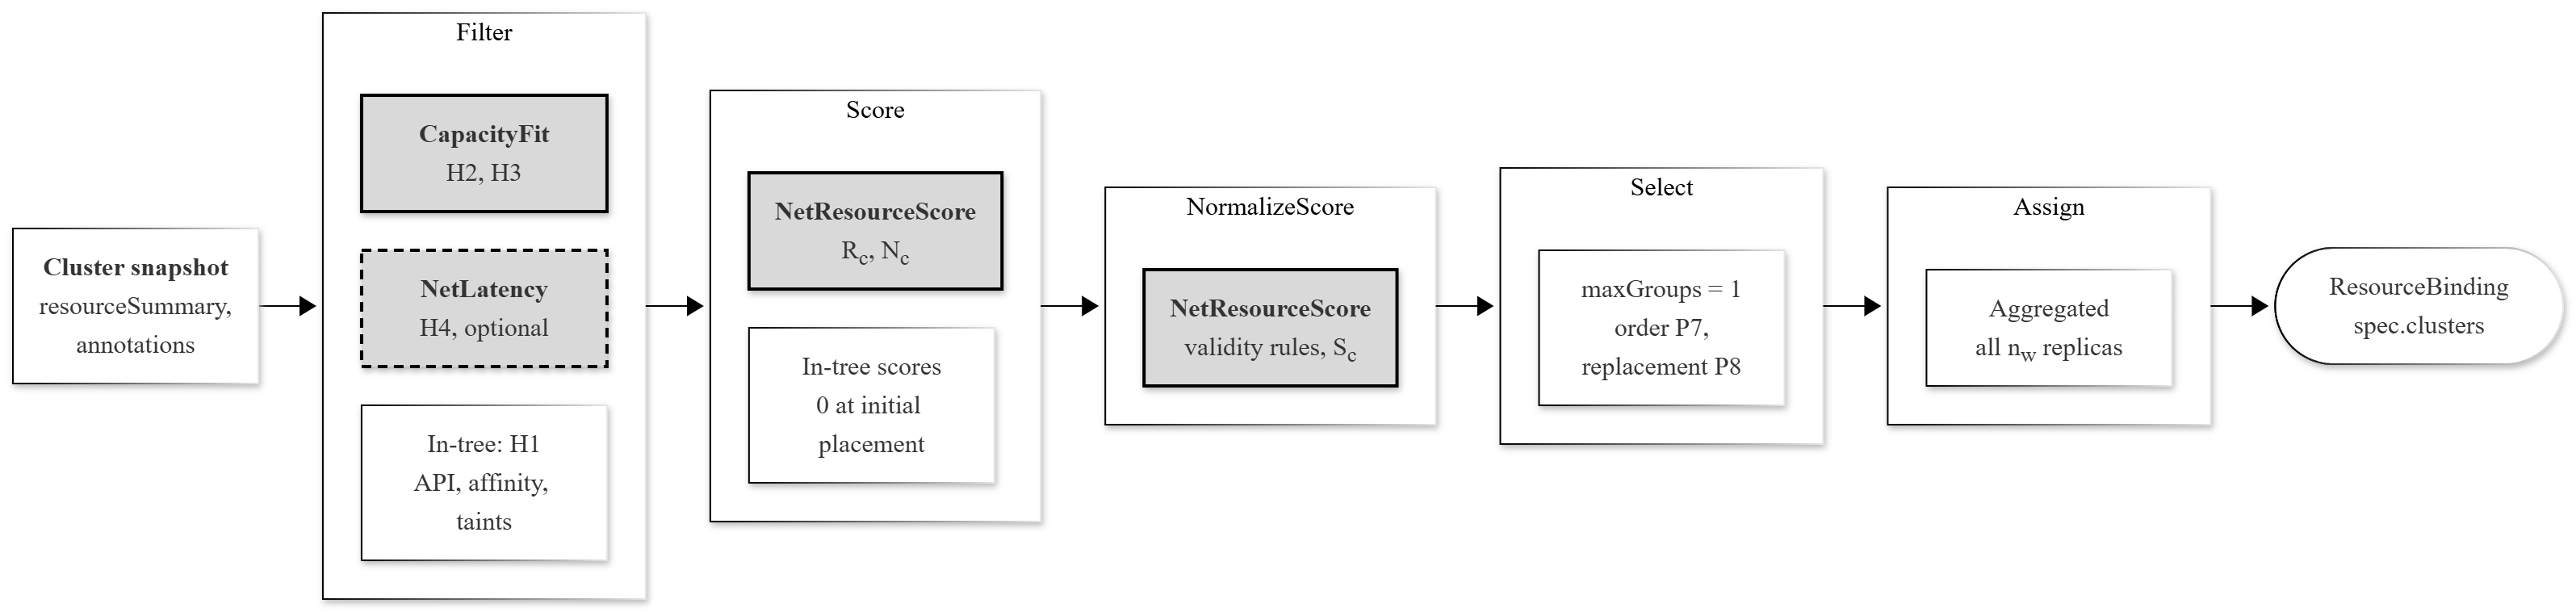
\includegraphics[width=\textwidth]{figures/pipeline.png}}% exported from figures/mermaid/pipeline.mmd
  {\resizebox{\textwidth}{!}{% Fig. 1 -- Karmada scheduling pipeline with the proposed plugins (shaded).
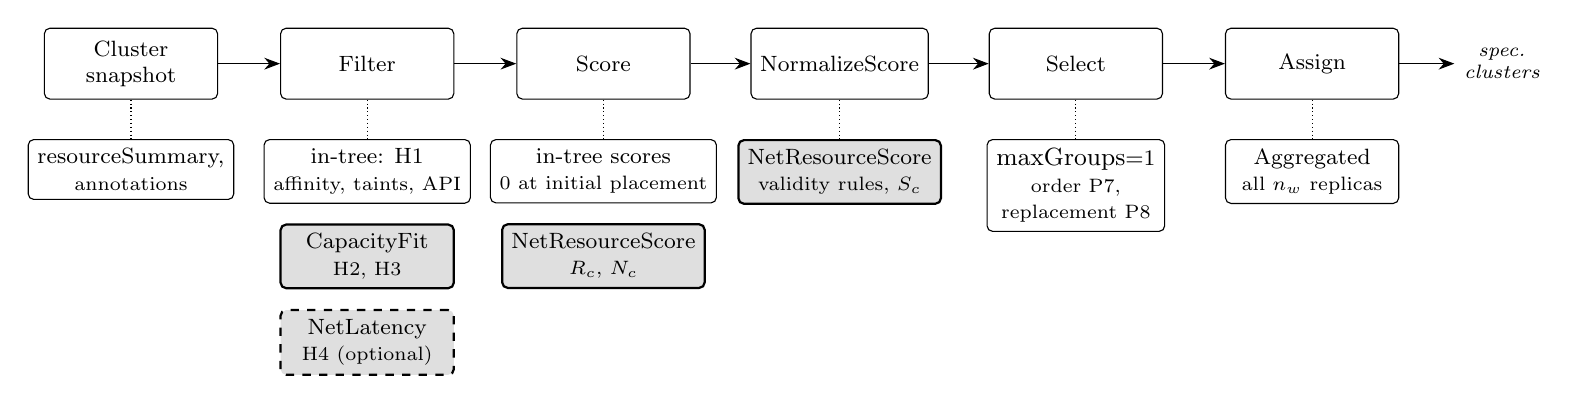
\begin{tikzpicture}[
  font=\footnotesize, >={Stealth[length=2mm]},
  stage/.style={draw, rounded corners=2pt, align=center, minimum width=2.2cm, minimum height=0.9cm, fill=white},
  prop/.style={draw, rounded corners=2pt, align=center, minimum width=2.2cm, minimum height=0.7cm, fill=gray!25, thick},
  exist/.style={draw, rounded corners=2pt, align=center, minimum width=2.2cm, minimum height=0.7cm, fill=white},
  lbl/.style={font=\scriptsize\itshape, align=center}
]
\node[stage] (snap) at (0,0) {Cluster\\snapshot};
\node[stage] (filt) at (3.0,0) {Filter};
\node[stage] (score) at (6.0,0) {Score};
\node[stage] (norm) at (9.0,0) {NormalizeScore};
\node[stage] (sel) at (12.0,0) {Select};
\node[stage] (asg) at (15.0,0) {Assign};

\foreach \a/\b in {snap/filt, filt/score, score/norm, norm/sel, sel/asg} \draw[->] (\a) -- (\b);
\draw[->] (asg.east) -- ++(0.7,0) node[right, lbl] {spec.\\clusters};

% plugins below each stage
\node[exist, below=0.5cm of filt] (f1) {in-tree: H1\\ \scriptsize affinity, taints, API};
\node[prop, below=0.25cm of f1] (f2) {CapacityFit\\ \scriptsize H2, H3};
\node[prop, dashed, below=0.25cm of f2] (f3) {NetLatency\\ \scriptsize H4 (optional)};
\node[exist, below=0.5cm of score] (s1) {in-tree scores\\ \scriptsize 0 at initial placement};
\node[prop, below=0.25cm of s1] (s2) {NetResourceScore\\ \scriptsize $R_c$, $N_c$};
\node[prop, below=0.5cm of norm] (n1) {NetResourceScore\\ \scriptsize validity rules, $S_c$};
\node[exist, below=0.5cm of sel] (sl1) {\code{maxGroups}=1\\ \scriptsize order P7,\\ \scriptsize replacement P8};
\node[exist, below=0.5cm of asg] (a1) {Aggregated\\ \scriptsize all $n_w$ replicas};
\node[exist, below=0.5cm of snap] (sn1) {resourceSummary,\\ \scriptsize annotations};

\foreach \s/\p in {snap/sn1, filt/f1, score/s1, norm/n1, sel/sl1, asg/a1} \draw[densely dotted] (\s.south) -- (\p.north);
\end{tikzpicture}
}}% TikZ fallback
\caption{Karmada scheduling stages and the position of the proposed plugins (shaded)}\label{fig:pipeline}
\end{figure}

\subsection{Algorithm}\label{sec:alg-algorithm}

\Cref{alg:netresource} gives the procedures of the three plugins. Score computes the resource term for each cluster separately, because Karmada calls it once per cluster. The validity rules of \cref{eq:score} depend on the whole candidate set, which in Karmada is visible only in the normalisation step (P1); the final score is therefore computed there. Every procedure returns a result for malformed input instead of an error.

\begin{algorithm}[t]
\caption{Filter, score and normalisation procedures of the proposed plugins}\label{alg:netresource}
\small\setstretch{1.0}
\begin{algorithmic}[1]
\Require binding with $n_w$, $d_w$; parameters $\alpha$, $\ell_{\mathrm{ref}}$, $\tau$, $q_{\min}$, vantage $v$, optional $\ell_{\max}$
\Procedure{CapacityFit}{$w, c$} \Comment{filter; H2, H3}
  \If{resource summary of $c$ is absent} \Return \textsc{Unschedulable} \EndIf
  \State $m \gets \min_{e \in E} e.\textsc{MaxAvailableReplicas}(c, w)$ \Comment{Karmada estimators}
  \If{$m < n_w$} \Return \textsc{Unschedulable} \EndIf
  \State \Return \textsc{Success}
\EndProcedure
\Procedure{NetLatency}{$w, c$} \Comment{optional filter; H4, fail-closed}
  \If{$\ell_{\max}$ not configured} \Return \textsc{Success} \EndIf
  \If{$\neg\,\textsc{Valid}(c, \mathrm{now})$ \textbf{or} $\ell_c > \ell_{\max}$} \Return \textsc{Unschedulable} \EndIf
  \State \Return \textsc{Success}
\EndProcedure
\Procedure{Score}{$w, c$} \Comment{called once per feasible cluster}
  \State $R \gets \operatorname{clip}\big(\min_{k} (A_c^k - U_c^k - P_c^k - n_w d_w^k)/A_c^k, 0, 1\big)$ \Comment{\cref{eq:resource}}
  \State \Return $\operatorname{round}(100 R)$ \Comment{provisional value}
\EndProcedure
\Function{Valid}{$c, t$}
  \State parse $\ell_c, t_c, q_c, v_c$ from the annotations of $c$; \textbf{if} parsing fails \Return \textbf{false}
  \State \Return $v_c = v \wedge q_c \geq q_{\min} \wedge t - t_c \leq \tau$ \Comment{\cref{eq:valid}}
\EndFunction
\Procedure{NormalizeScore}{list $L$ of (cluster, score)} \Comment{sees all candidates}
  \State $\Vset \gets \{ c \in L : \textsc{Valid}(c, \mathrm{now}) \}$
  \For{each $c \in L$}
    \State recompute $R_c$ from the snapshot \Comment{avoids rounding twice}
    \If{$\Vset = \emptyset$} $S_c \gets \operatorname{round}(100 R_c)$ \Comment{resource-only fallback; counted in a metric}
    \Else
      \State $N_c \gets \operatorname{clip}(1 - \ell_c/\ell_{\mathrm{ref}}, 0, 1)$ \textbf{if} $c \in \Vset$ \textbf{else} $0$ \Comment{missing is never favourable}
      \State $S_c \gets \operatorname{round}\big(100[\alpha R_c + (1-\alpha) N_c]\big)$
    \EndIf
  \EndFor
  \State \Return \textsc{Success}
\EndProcedure
\end{algorithmic}
\end{algorithm}

\subsection{Integration and configuration}\label{sec:alg-config}

The plugins are registered in a custom build of the Karmada scheduler through the out-of-tree registration function, and the parameters are passed as command-line options of that binary (P2) \cite{karmada_docs_custom_scheduler}. Because the score plugins are summed without weights (P3), the weighting of resource and network suitability is computed inside NetResourceScore and not by combining two plugins. The in-tree plugins remain enabled. At initial placement their scores are zero (P5), so the total score equals $S_c(w)$, and on a later rescheduling the existing locality preference of Karmada continues to apply unchanged.

Several scheduler instances can run side by side, each with its own scheduler name and leader-election lock \cite{karmada_docs_custom_scheduler}. This allows the same Karmada installation to offer the default behaviour, a resource-only configuration ($\alpha = 1$) and resource- and network-aware configurations ($0 < \alpha < 1$). A workload selects a configuration through the scheduler name in its PropagationPolicy, and removing the name returns it to the default scheduler. The same mechanism provides the comparison setting of the validation plan in \cref{sec:validation}.

Two configuration details affect correctness. First, when resource models are enabled with the default grades, clusters composed of small nodes are underestimated (\cref{sec:method-capacity}); such installations should define finer models or enable the accurate estimator. Second, until the pods of a newly placed workload appear in the member cluster, its demand is absent from the resource summary. Karmada can account for such in-flight placements through a feature gate that is alpha and disabled by default in v1.19.1. Without it, several placements made within one status interval may select the same cluster. This affects the default scheduler in the same way.

\section{Design Analysis and Discussion}\label{sec:analysis}

This section analyses the decisions that the design produces. The example below uses chosen input values to illustrate the decision rules. The values are not measurements, and the example makes no statement about response time or resource utilisation, which can only be established experimentally (\cref{sec:validation}).

\subsection{Illustrative scenario with conflicting criteria}\label{sec:analysis-example}

Three single-node member clusters, called edge, regional and central, are described in \cref{tab:example}. A workload with $n_w = 4$ replicas requests 250 millicores of CPU and 512 MiB of memory per replica, i.e.\ 1000 millicores and 2 GiB in total. The parameters are $\ell_{\mathrm{ref}} = 100$ ms and, for strategy C, $\alpha = 0.5$; all measurements are valid. Because the clusters have a single node, the aggregate summary path of the estimator applies without fragmentation, and $m_c(w) = \min_k \lfloor F_c^k / d_w^k \rfloor$.

\begin{table}[t]
\caption{Illustrative cluster states (chosen inputs, not measurements) and resulting values}\label{tab:example}
\centering\small\setstretch{1.0}
\begin{tabularx}{\textwidth}{@{}LCCC@{}}
\toprule
\textbf{Quantity} & \textbf{edge} & \textbf{regional} & \textbf{central} \\
\midrule
$A^{\mathrm{cpu}}$ (m) / $A^{\mathrm{mem}}$ (GiB) & 4000 / 8 & 8000 / 16 & 16000 / 32 \\
$F^{\mathrm{cpu}}$ (m) / $F^{\mathrm{mem}}$ (GiB) & 1200 / 3 & 4000 / 8 & 12000 / 24 \\
$\ell_c$ (ms) & 5 & 25 & 60 \\
$m_c(w)$ (replicas), H2 satisfied & 4, yes & 16, yes & 48, yes \\
$R_c(w)$, \cref{eq:resource} & 0.050 & 0.375 & 0.688 \\
$N_c$, \cref{eq:network} & 0.95 & 0.75 & 0.40 \\
$S_c(w)$ with $\alpha = 0.5$, \cref{eq:score} & 50 & 56 & 54 \\
\bottomrule
\end{tabularx}
\end{table}

The four configurations of the extended scheduler select different clusters. The default scheduler (A) gives every cluster a score of zero (P5) and therefore selects central, which has the largest number of available replicas (P7). The resource-only configuration (B, $\alpha = 1$) also selects central, because central has the largest relative headroom. The combined configuration (C, $\alpha = 0.5$) selects regional. A latency-only configuration ($\alpha = 0$) would select edge, which is closest to the clients but would retain only 5\,\% of its CPU as free requestable capacity after the placement. In this example, C avoids both the cluster with the least headroom and the most distant cluster. Whether this choice leads to lower response times than A or B depends on how the workload behaves under load at each cluster, which the validation in \cref{sec:validation} is designed to measure.

\subsection{Sensitivity to the weight}\label{sec:analysis-weight}

For fixed cluster states, every score in \cref{eq:score} is linear in $\alpha$. In the example, $S_{\mathrm{edge}}/100 = 0.95 - 0.900\,\alpha$, $S_{\mathrm{regional}}/100 = 0.75 - 0.375\,\alpha$ and $S_{\mathrm{central}}/100 = 0.40 + 0.2875\,\alpha$. Equating the lines gives two switching points: edge is selected for $\alpha < 0.381$, regional for $0.381 < \alpha < 0.528$ and central for $\alpha > 0.528$ (\cref{fig:regions}). Integer rounding can move a switching point by up to one score point. Two properties follow. First, for any cluster state the selection changes only at a finite number of values of $\alpha$, which can be computed in advance; this makes the behaviour of a configuration predictable (D-R5). Second, the width of the intermediate region depends on the cluster states, so a single $\alpha$ is not optimal for all situations. The switching points also give concrete predictions that an experiment can test.

\begin{figure}[t]
\centering
% Fig. 3 -- Score of each cluster as a function of alpha for the illustrative scenario of Tab. 6.
% Analytic lines from Eq. (score); no measured data.
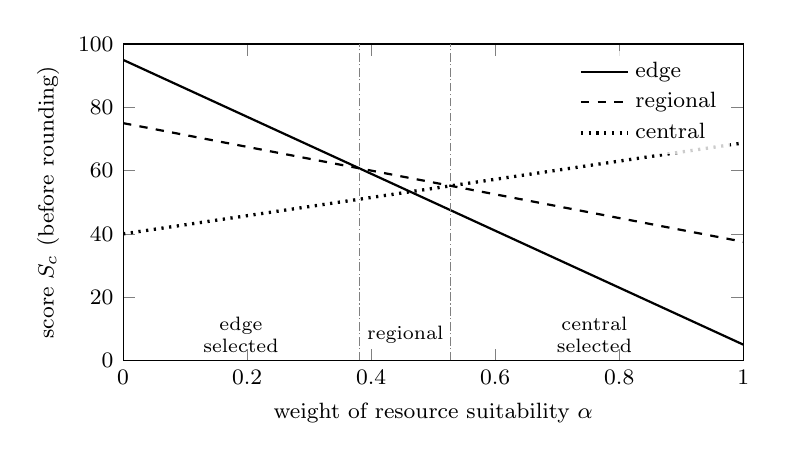
\begin{tikzpicture}
\begin{axis}[
  width=0.78\textwidth, height=5.6cm,
  xmin=0, xmax=1, ymin=0, ymax=100,
  xlabel={weight of resource suitability $\alpha$}, ylabel={score $S_c$ (before rounding)},
  xtick={0,0.2,0.4,0.6,0.8,1}, ytick={0,20,40,60,80,100},
  legend style={at={(0.98,0.98)}, anchor=north east, font=\footnotesize, draw=none, fill=white, fill opacity=0.8, text opacity=1},
  legend cell align=left,
  tick label style={font=\footnotesize}, label style={font=\footnotesize},
  every axis plot/.append style={thick, samples=2, domain=0:1},
]
\addplot[black, solid]        {100*(0.95 - 0.900*x)};  \addlegendentry{edge}
\addplot[black, dashed]       {100*(0.75 - 0.375*x)};  \addlegendentry{regional}
\addplot[black, dotted, very thick] {100*(0.40 + 0.2875*x)}; \addlegendentry{central}
\draw[gray, densely dashdotted] (axis cs:0.381,0) -- (axis cs:0.381,100);
\draw[gray, densely dashdotted] (axis cs:0.528,0) -- (axis cs:0.528,100);
\node[font=\scriptsize, align=center] at (axis cs:0.19,8) {edge\\selected};
\node[font=\scriptsize, align=center] at (axis cs:0.455,8) {regional};
\node[font=\scriptsize, align=center] at (axis cs:0.76,8) {central\\selected};
\end{axis}
\end{tikzpicture}

\caption{Score of each cluster in the scenario of Tab.~\ref*{tab:example} as a function of $\alpha$ (analytic, no measured data)}\label{fig:regions}
\end{figure}

\subsection{Behaviour with missing and stale measurements}\label{sec:analysis-missing}

\Cref{tab:missing} applies the validity rules of \cref{sec:method-validity} to the same scenario. When only the measurement of regional is stale, regional obtains $N = 0$ and is no longer preferred; the stale value neither helps nor removes the cluster. When all measurements are stale, the scheduler behaves exactly like the resource-only configuration. When the optional hard bound H4 is used with $\ell_{\max} = 30$ ms, central becomes ineligible and the remaining clusters are ranked as before.

\begin{table}[t]
\caption{Selection in the scenario of Tab.~\ref*{tab:example} under missing data and a hard bound ($\alpha = 0.5$)}\label{tab:missing}
\centering\small\setstretch{1.0}
\begin{tabularx}{\textwidth}{@{}LCC@{}}
\toprule
\textbf{Condition} & \textbf{Scores (edge, regional, central)} & \textbf{Selected} \\
\midrule
All measurements valid & 50, 56, 54 & regional \\
Measurement of regional stale & 50, 19, 54 & central \\
All measurements stale (fallback) & 5, 38, 69 & central \\
Hard bound $\ell_{\max} = 30$ ms (H4) & 50, 56, ineligible & regional \\
\bottomrule
\end{tabularx}
\end{table}

\subsection{Complexity and overhead}\label{sec:analysis-complexity}

For $|\Cset|$ clusters and $|\Kr|$ resources, the score and normalisation procedures perform $O(|\Cset|\,|\Kr|)$ arithmetic operations and read only the in-memory snapshot. The capacity filter calls each registered estimator once per cluster. With the general estimator this is a local computation; the accurate estimator adds a remote call per decision. Karmada already calls the estimators in its selection stage, so the filter repeats an existing computation rather than adding a new kind of cost. The probe costs one measurement and one annotation update per cluster and period, outside the scheduling path. These are analytical statements; the actual overhead has to be measured (\cref{sec:validation}).

\subsection{Design decisions and trade-offs}\label{sec:analysis-tradeoffs}

The design keeps Karmada's own stages and adds information instead of replacing the decision procedure. Compared with an external optimiser \cite{tabatabaei2025cnf}, it gives up global optimality across several workloads in exchange for a closed-form score that is evaluated in the existing pipeline. Compared with a scheduler that replaces Karmada's cluster selection \cite{bregar2026cosmospan}, it gives up joint selection of cluster and node in exchange for compatibility with Karmada's policies, estimators and default behaviour.

Reusing Karmada's estimators for the capacity condition makes the filter consistent with the selection stage, but it also inherits the estimators' limitations: an optimistic aggregate estimate on clusters with several nodes, or a conservative estimate with coarse resource models. Using the request-based resource summary avoids a dependency on a monitoring system, at the cost of ignoring unrequested load. Treating missing measurements pessimistically prevents an unmeasured cluster from being preferred, but a cluster whose probe fails is disadvantaged even if it is close to the clients; the fallback limits this effect to the case of partial failure. Annotations avoid scheduling churn but are not versioned, so the probe and the scheduler have to agree on the schema. Finally, the single client vantage point keeps the model simple but represents only one client population; several populations would require one measurement per population and a way for a workload to name its population.

\section{Proposed Experimental Validation for Future Research}\label{sec:validation}

The design has not been implemented or measured. This section defines the experimental study that will test it as part of subsequent work.

\emph{Questions.} The study will answer four questions: (V1) whether the network term changes the response-time distribution relative to the resource-only and default configurations when all clusters have sufficient capacity; (V2) whether, when the cluster closest to the clients has little headroom, the combined score avoids the saturation that latency-only selection causes, and at which latency cost; (V3) whether selection under stale and missing measurements follows \cref{tab:missing}; and (V4) how much time the plugins add per decision and how this grows with the number of clusters.

\emph{Compared configurations.} The study compares the default scheduler (A), the resource-only configuration (B, $\alpha = 1$), the combined configuration (C, $\alpha \in \{0.25, 0.5, 0.75\}$) and a latency-only ablation ($\alpha = 0$). For a fair comparison, all configurations use the same workloads, the same PropagationPolicy (divided, aggregated, one cluster), the same estimator settings and the same clusters, and they differ only in the scheduler name.

\emph{Environment.} A Karmada control plane manages three member clusters with different allocatable resources, created with a lightweight Kubernetes distribution on local virtual machines. Client-to-cluster delay is emulated with the Linux traffic-control queueing discipline netem, load is generated with k6, and observations are collected with Prometheus. Workloads declare resource requests, which the estimators require, and are CPU-bound with limits, so that saturation affects their response time.

\emph{Scenarios.} Five scenarios are planned: heterogeneous capacity without pressure; CPU and memory pressure on one cluster; latency degradation on one cluster; the conflict of \cref{sec:analysis-example}, with the closest cluster having the least headroom; and stale or missing measurements, produced by stopping the probe for one cluster and then for all clusters.

\emph{Metrics.} Response time at the 50th, 95th and 99th percentiles and the rate of responses exceeding a response-time objective \cite{dean2013tail}; the selected cluster per run; the share of requested resources per cluster; measured CPU and memory utilisation for observation; and decision time from the scheduler's duration metrics for plugins and complete scheduling attempts \cite{karmada_repo}, complemented by micro-benchmarks for 3 to 100 synthetic clusters, since the shortest histogram bucket of these metrics is 1 ms.

\emph{Protocol and analysis.} Each combination of scenario and configuration will be repeated at least ten times in randomised order, with a warm-up period, a fixed measurement window and a reset of the environment between runs. Percentiles will be computed per run and summarised by their median over runs with bootstrap confidence intervals; differences will be tested with non-parametric tests and reported with effect sizes, including results that show no difference. The reporting will follow the methodological principles for reproducible performance evaluation in cloud computing \cite{papadopoulos2021methodological}.

\emph{Threat to validity.} With emulated delay, part of any latency reduction exists by construction, because the scheduler avoids the clusters to which delay was added. The analysis will therefore relate observed differences to the emulated ones and concentrate on the conflict scenario, in which proximity and capacity pull in opposite directions.

\section{Limitations}\label{sec:limitations}

The paper presents a design, not an evaluated system. No claim is made that the design improves response time or resource utilisation; such claims require the study of \cref{sec:validation}.

The analysis of Karmada refers to release v1.19.1. Several of the properties in \cref{tab:karmada}, such as the unweighted sum of scores and the replacement rule in the selection stage, are internal behaviour rather than documented interfaces and may change in later releases. The analysis has to be repeated for each release on which the design is implemented.

The resource term uses requested resources and aggregate values. It does not see load from pods without requests, and its accuracy for the capacity condition is limited by the configured estimator. The network term uses one client vantage point and the round-trip time to the cluster entry point; it does not cover several client populations, bandwidth, or latency between services of a workload split across clusters, which single-cluster placement excludes by assumption. The freshness check compares timestamps written by the probe with the scheduler's clock and assumes synchronised clocks.

The design concerns initial placement only. Because Karmada does not revisit placements when cluster conditions change (P11), a workload stays on the selected cluster even if the conditions that led to the decision no longer hold.

\section{Conclusions and Future Work}\label{sec:conclusions}

The paper designed a cluster selection strategy that adds client-to-cluster latency to Karmada's scheduling without replacing Karmada's own stages. Regarding RQ1, the analysis of the Karmada v1.19.1 source code showed that a custom objective has to be computed inside a single score plugin, that it only takes effect together with a cluster spread constraint, and that Karmada's default behaviour for a new single-cluster workload already prefers the cluster with the most available replicas. Regarding RQ2, mandatory conditions are evaluated in the filter stage, and the capacity condition reuses Karmada's replica estimators so that it agrees with the selection stage. Regarding RQ3, a network measurement contributes to the score only if it is recent and based on enough samples; a missing measurement is treated as the least favourable value, and the score falls back to resource-only ranking when no candidate has a valid measurement. Regarding RQ4, the design trades global optimality and joint node selection for compatibility with Karmada and a closed-form score whose decisions can be predicted, and it inherits the limitations of request-based capacity information.

Future work consists of implementing the plugins and the latency probe, and carrying out the experimental validation of \cref{sec:validation} against the default and resource-only configurations. Further extensions are the rebalancing of workloads when conditions change, which Karmada supports only through explicit triggers \cite{karmada_docs_rebalancer}; the use of measured utilisation alongside requested resources; several client populations; latency between services for workloads split across clusters; and an evaluation of performance, scalability and reliability on larger installations.


\printbibliography[heading=csmd]

\end{document}
